
\documentclass{article}

\usepackage[ngerman]{babel}                     %for german umlauts
\usepackage[utf8]{inputenc}
\usepackage{subfigure}
\usepackage{float}
\usepackage[bw,framed,autolinebreaks,useliterate]{mcode}
% \usepackage[ansinew]{inputenc}        %for german umlauts

\usepackage{graphicx}
\usepackage{hyperref}

\usepackage{amssymb}    %for different fonts
\usepackage{amsmath}
% Geht nicht: \usepackage{bbm}
% \usepackage[usenames,dvips]{color} %only way to get it running with pdf:(
% \usepackage[pdftex,usenames,dvipsnames]{color}        % does not work
% \usepackage{color}
\usepackage{verbatim}
\usepackage{polynom}

\setlength{\parindent}{0pt}
\addtolength{\hoffset}{-2cm}
\addtolength{\voffset}{-1cm}
\addtolength{\textheight}{3cm}
\addtolength{\textwidth}{3cm}

\newcommand{\im}{\operatorname{Im}}
\newcommand{\rg}{\operatorname{rg}}
\newcommand{\ggt}{\operatorname{ggT}}

\begin{document}

\section*{\begin{center} Mustererkennung - Aufgabenblatt 05 \end{center}}
\begin{center}
  André Hacker und Dimitri Schachmann \\
\end{center}


\subsection*{1. Ridge Regression}
Für diese Aufgabe haben wir zunächst die Daten entsprechend der Aufgabenstellung
normiert:
\begin{lstlisting}
% Standardize data by subtracting the mean and deviding by the standard
% deviation
function r = standardize(samples)
  m = mean(samples);
  sd = std(samples);
  for i = 1:size(samples,1)
    samples(i,:) = (samples(i,:) - m) ./ sd;
  end
  r = samples;
end
\end{lstlisting}

Das Einlesen der Daten sieht dann entsprechend wie folgt aus.
\begin{lstlisting}
tra = standardize(dlmread('prostate-tra.mat', ' '));
trates = standardize(dlmread('prostate-all.mat', ' '));
\end{lstlisting}
Unsere Funktion für die Berechnung der ridge regression sieht wie folgt aus:
\begin{lstlisting}
% Computes the ridge regression parameters
function a = ridgeRegression(y, samples, lambda)
  a = [];
  for i = 1:size(lambda,2)
    t = inv(samples'*samples + (lambda(:,i)*eye(size(samples'*samples))));
    a = [a (t * samples'*y)];
  end
end
\end{lstlisting}
Schließlich haben wir das Ergebnis grafisch dargestellt mit der folgenden
funktion:
\begin{lstlisting}
% plot the ridge regression
function r = plotRidgeRegression(y, samples, labels, filename)
  k = [0:1:1000 30000];
  data = ridgeRegression(y,samples,k);
  plt = figure();
  xlim([-1 8]);
  ylim([-0.3 0.7])
  hold on;
  plot(df(samples,k), data,'LineWidth',2,'Color','blue');
  for i = 1:size(labels,1)
    text(size(data,1)+0.1, data(i,1) ,labels(i,:),'FontSize',10);
  end
  line([-1 8],[0 0], 'Color', 'black')
  xlabel('df(\lambda)', 'FontSize', 17);
  ylabel('Coefficients', 'FontSize', 17);
  print(plt,'-depsc',[filename '.eps']);
end
\end{lstlisting}
Die Funktion für die effektiven Freiheitsgrade haben wir von Hastie (2011):
\begin{lstlisting}
% df(l) function from Hastie
function r = df(samples, lambda)
  r = [];
  for i = 1:size(lambda,2)
    t = inv(samples'*samples + (lambda(:,i)*eye(size(samples'*samples))));
    a = samples * t * samples';
    r = [r trace(a)];
  end
end
\end{lstlisting}

Das Ergebnis sieht dann mit den Trainingsdaten so wie im Buch aus:
\begin{figure}[H]
  \begin{subfigure}
    \centering
    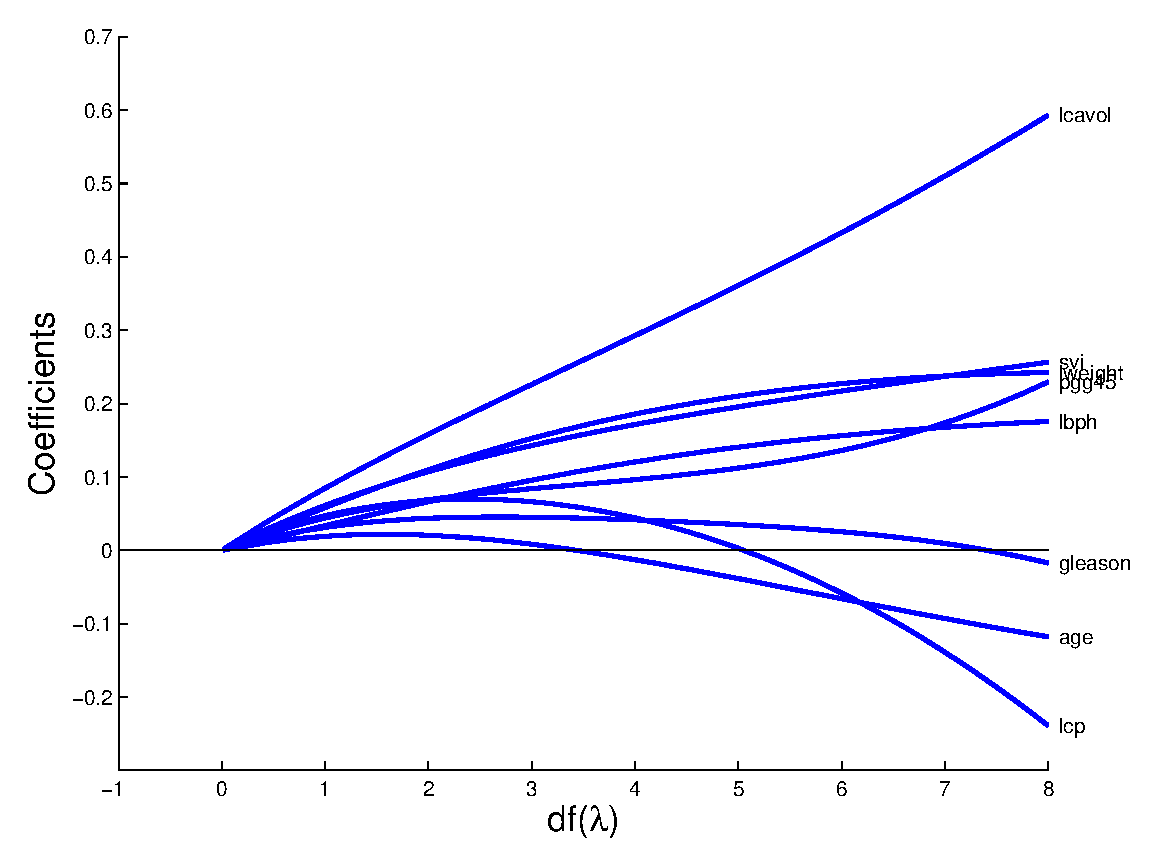
\includegraphics[scale=0.75]{ridgeregression-tra.eps}
  \end{subfigure}
\end{figure}
\newpage
Wenn wir alle Samples verwenden, dann sieht das wie folgt aus:
\begin{figure}[H]
  \begin{subfigure}
    \centering
    \includegraphics[scale=0.75]{ridgeregression-all.eps}
  \end{subfigure}
\end{figure}


\subsection*{2. Bootstrap}
Für den Bootstrap Algorithmus lesen wir alle prostate Daten aus und wählen dort
nur die Merkmale 1, 5 und 7 aus.
\begin{lstlisting}
  % read the ALL of the data
  all = dlmread('prostate-all.mat', ' ');

  % we consider only features 1, 5 and 7
  testn = all(1:10,[1 5 7]);

  % Add 1 dimension for offset/bias
  testn = [ones(size(testn, 1),1) testn];
\end{lstlisting}
Als nächstes wird in einer Schleife für verschiedene Proben der Bootstrap
Algorithmus durchgeführt:
\begin{lstlisting}
  q = 50;   % number of sample picks per iteration
  bootstraps = [];
  for i = 1:100
    % pick 50 random indecies
    ran = randi([1,size(all,1)],q,1);
    % get the samples at the random indecies
    allIn  = all(ran,[1 5 7]);
    % get the actual values at the indecies
    allOut = all(ran,9);
    % Add 1 dimension for offset/bias
    allIn = [ones(size(allIn, 1),1) allIn];
    % compute linear regression and add to bootstrap list
    bootstraps = [bootstraps getWeightsLeastSquares(allIn, allOut)];
  end
\end{lstlisting}
Für die Berechnung der linearen regression verwenden wir unsere alte Funktion:
\begin{lstlisting}
% Least Squares Fitting based on samples and output column vector
function w = getWeightsLeastSquares(samples, y)
  % Compute pseudo-inverse matrix
  pseudo = getPseudoInverse(samples);
  w = pseudo * y;
end

% Get pseudo-inverse matrix, needed for least squares fitting
function p = getPseudoInverse(X)
  % very likely that inverse exists if we have many samples
  p = inv(X' * X) * X';
end
\end{lstlisting}
Für die Bestimmug des Mittelwertes und des Konfidenzintervals für verschiedene
Proben, haben wir eine Funktion geschrieben:
\begin{lstlisting}
% use bootstraped data for prediction
function [m d] = computeConfidence(bootstraps, y)
  m = [];
  d = [];
  for i = 1:size(y,1)
    p = [];
    for j = 1:size(bootstraps,2)
      p = [p predict(bootstraps(:,j), y(i,:))];
    end
    m = [m ; mean(p)];
    d = [d ; 2*std(p)];
  end
end

% Predicts value for input based on weights
% samples = list of row vectors
% weights = column-vector
function r = predict(weights, samples)
  r = samples * weights;
end
\end{lstlisting}
Das haben wir dann auf die ersten 10 Samples aus den Daten angewendet.
\begin{lstlisting}
  [m d] = computeConfidence(bootstraps, testn);
  fid = fopen('task2-results.txt','w');
  fprintf(fid, 'Mean and 2*standard deviation for the first %d samples\n', ...
          size(testn,1));
  for i = 1:size(testn,1)
    fprintf(fid, 'Sample %d\t| Mean = %f | confidence =  %f\n', i, m(i,:),d(i,:));
  end
\end{lstlisting}
Das Ergebnis davon ist im folgenden zu sehen:
\begin{samepage}
\verbatiminput{task2-results.txt}
\end{samepage}
\subsection*{3. Experiment}
Wir haben das Experiment wie beschrieben durchgeführt, also einen
zufälligen 16$\times$1 Vektor wiederholt mit der Kovarianzmatrix einer
Ziffer multipliziert. Ziwschendurch haben wir jedes mal auf 1
normiert. Hier beispielsweise für die Ziffer 8:
\begin{lstlisting}
  eight = load('pendigits8.txt');
  eight = eight(:,1:end-1);
  [m covarianceMatrix] = meanAndCov(eight);
  covarianceMatrix = covarianceMatrix/norm(covarianceMatrix);
  ran = randi([1,100],16,1)';
  ran = ran/norm(ran);
  for i = 1:10
    ran = ran * covarianceMatrix;
    ran = ran/norm(ran);
  end
\end{lstlisting}
\begin{samepage}
In der Vorlesung haben wir gelernt, dass ran jetzt den längsten
Eigenvektor der Kovarianzmatrix enthalten sollte. Das haben wir mit
der eig() Funktion von Matlab überprüft:
\begin{lstlisting}
  [eigenvectors, eigenvalues] = eig(covarianceMatrix);
  pc =eigenvectors(:,end)';
  fid = fopen('task3-results.txt','w');
  fprintf(fid, 'experiment. result \t| longest eigenvector\n');
  fprintf(fid, '-------------------------------------\n');
  for i = 1:size(ran,2)
    fprintf(fid, '%+.3f\t\t|\t%+.3f\n',ran(:,i),pc(:,i));
  end
\end{lstlisting}
\end{samepage}
\begin{samepage}
Und tatsächlich sieht das Ergebnis wie folgt aus:
\verbatiminput{task3-results.txt}
\end{samepage}
\end{document}